%%%%%%%%%%%%%%%%%%%%%%%%%%%%%%%%%%%%%%%%%%%%%%%%%%%%%%
% This is beamer setup. Not required for extraction. I personnaly like the default barebones style.
\documentclass{beamer}
\usepackage[utf8]{inputenc}
\usetheme{default}

%%%%%%%%%%%%%%%%%%%%%%%%%%%%%%%%%%%%%%%%%%%%%%%%%%%%%%
\usepackage{tikz}
\usepackage{bbm}
\usepackage{amsmath}
\usepackage{hyperref}

\newcommand\Shifted[2]{\Delta_{#1}(#2)}
\newcommand\Reversed[1]{\overline{#1}}

\newcommand\SymSquare{\begin{tikzpicture}[baseline=0.5ex]%
        \draw (0,0) -- (0,1em) -- (1em,1em) -- (1em,0) -- cycle;
\end{tikzpicture}}
\newcommand\Indicator[1]{\SymSquare(#1)}

\newcommand\SymPositiveTriangle{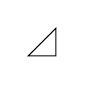
\begin{tikzpicture}[baseline=0.5ex]%
        \draw (0,0) -- (1em,0em) -- (1em,1em) -- cycle;
\end{tikzpicture}}
\newcommand\PositiveTriangle[1]{\SymPositiveTriangle(#1)}

\newcommand\SymNegativeTriangle{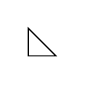
\begin{tikzpicture}[baseline=0.5ex]%
        \draw (0,0) -- (0,1em) -- (1em,0em) -- cycle;
\end{tikzpicture}}
\newcommand\NegativeTriangle[1]{\SymNegativeTriangle(#1)}

\newcommand\SymTrapezoid{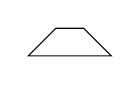
\begin{tikzpicture}[baseline=0.5ex]%
        \draw (0,0) -- (3em,0) -- (2em,1em) -- (1em,1em) -- cycle;
\end{tikzpicture}}
\newcommand\Trapezoid[2]{\SymTrapezoid(#1,#2)}% Trapezoid(h,b)

\newcommand\D{\mathrm{d}}
\newcommand\Convolution{\ast}
\newcommand\Correlation{\star}
\newcommand\IntR[2]{\int_{-\infty}^{\infty}#1 \D#2}
\newcommand\Equiv{\Leftrightarrow}
\newcommand\Then{\Rightarrow}
\renewcommand\And{\wedge}

% \GridAxis{from_x}{to_x}{from_y}{to_y}
\newcommand\GridAxis[4]{%
    \draw[very thin,color=gray] (#1,#3) grid (#2,#4);
    \draw[->] (#1,0) -- (#2,0) node[right] {$x$};
    \draw[->] (0,#3) -- (0,#4);
    \node[below right] at (0,0) {$0$};
    \coordinate (Origin) at (0,0);
    \coordinate (FuncStart) at (#1,0);
    \coordinate (FuncEnd) at (#2,0);
}
\newcommand\SizedGridAxis[4]{%
    \GridAxis{#1}{#2}{#3}{#4}
    \node[below right] at (0,1) {$1$};
    \node[below right] at (1,0) {$1$};
}
%%%%%%%%%%%%%%%%%%%%%%%%%%%%%%%%%%%%%%%%%%%%%%%%%%%%%%

\begin{document}

\begin{frame}{Hawkes implementation}
    \begin{itemize}
        \item Summary
            \begin{itemize}
            \item C++14 tool
            \item Input: BED format files + region names
            \item Output: estimator coefficients as text format matrix
        \end{itemize}
        \item Parameters
        \begin{itemize}
            \item $M$ : number of processes
            \item $K$ : function base size (for $\varphi_k$)
            \item $N_l$ : set of points of process $l$ ; $x_l \in N_l$ is a point.
        \end{itemize}
        \item Regions are independent : algorithms handle one region
        \item Implemented cases

        \begin{tabular}{|c|c|c|c|} \hline
            \textbf{Base} & \textbf{Kernel} & \textbf{Time (PRDM9)} \\ \hline
            histogram & & 566 ms \\ \hline
            histogram & intervals & 1.1 s \\ \hline
        \end{tabular}
    \end{itemize}
\end{frame}

\begin{frame}{Computed values}
    \begin{itemize}
        \item No kernel
        \begin{itemize}
            \item $B_{l,k}^m = \sum_{x_l,x_m} \varphi_k (x_m - x_l)$
            \item $g_{l,k} = \int \sum_{x_l} \varphi_k (x - x_l) dx$
            \item $\mathsf{G}_{l,k,k'}^{l'} = \int (\sum_{x_l} \varphi_k (x - x_l)) (\sum_{x_{l'}} \varphi_{k'} (x - x_{l'})) dx$
            \item $\hat{B}_{l,k}^m = \sup_x \sum_{x_l} \varphi_k (x - x_l)$
        \end{itemize}
        \item With kernels
        \begin{itemize}
            \item $B_{W,l,k}^m = \sum_{x_l,x_m} [ W_l \Convolution W_m \Convolution \varphi_k ] (x_m - x_l)$
            \item $g_{W,l,k} = \int \sum_{x_l} [ W_l \Convolution \varphi_k ] (x - x_l) dx$
            \item $\mathsf{G}_{W,l,k,k'}^{l'} = \int (\sum_{x_l} [ W_l \Convolution \varphi_k ] (x - x_l)) (\sum_{x_{l'}} [ W_{l'} \Convolution \varphi_{k'} ] (x - x_{l'})) dx$
            \item $\hat{B}_{W,l,k}^m = \sup_x \sum_{x_l} [ W_l \Convolution W_m \Convolution \varphi_k ] (x - x_l)$
        \end{itemize}
    \end{itemize}
\end{frame}

\begin{frame}{General value properties}
    \begin{itemize}
        \item $g_{l,k}$ and $g_{W,l,k}$ are simple to compute
        \[ g_{l,k} = \int \sum_{x_l} \varphi_k (x - x_l) dx = |N_l| \int \varphi_k(x) dx \]
        \[ g_{W,l,k} = |N_l| \int [ W_l \Convolution \varphi_k ] = |N_l| \int W_l \int \varphi_k \]

        \item $\mathsf{G}$ is symmetric : $\mathsf{G}_{l,k,k'}^{l'} = \mathsf{G}_{l',k',k}^{l}$, same with kernel

        \item If $\varphi_k$ is the histogram base :
        \begin{itemize}
            \item $\mathsf{G}_{l,k,k'}^{l'} = \mathsf{G}_{l,k+c,k'+c}^{l'}$ (substitution  $x \rightarrow x + \delta c$)
            \item $\mathsf{G}_{W,l,k,k'}^{l'} = \mathsf{G}_{W,l,k+c,k'+c}^{l'}$ (subtitution and convolution properties)
            \item $\mathsf{G}_{l}^{l'}$ values cost $2K+1$ computations instead of $K^2$
        \end{itemize}
    \end{itemize}
\end{frame}

\begin{frame}{Case histogram, no kernel}
    Specialized algorithms based on $\mathbbm{1}_{]k\delta, (k+1)\delta]} = \varphi_k \sqrt{\delta}$.

    \[ B_{l,k}^m \sqrt{\delta} = \sqrt{\delta} \sum_{x_l,x_m} \varphi_k (x_m - x_l) =\sqrt{\delta}  \sum_{x_l} \sum_{x_l + k\delta < x_m \le x_l +(k+1)\delta} 1 \]

    Algorithm
    \begin{itemize}
        \item Compute position of $\min\{x_m,  x_m > x_l + k\delta\}$ in $N_m$ : $P(x_l,k)$.
        \item $\sum_{x_l + k\delta < x_m \le x_l +(k+1)\delta} 1 = P(x_l,k+1) - P(x_l,k)$
        \item $x_l \le x'_l \Rightarrow P(x_l,k) \le P(x'_l, k)$, we can scan from previous $P(x_l,k)$ when looking at the next $x_l$
    \end{itemize}

    Complexity (single, all) : $\mathcal{O}( |N_l| + |N_m| )$, $\mathcal{O}( M^2 K \max|N| )$
\end{frame}

\begin{frame}{Case histogram, no kernel (2)}
    \begin{block}
        {$F_{l,k}(x) = \sum_{x_l} \mathbbm{1}_{]k\delta, (k+1)\delta]} (x - x_l) = \sum_{x_l} \mathbbm{1}_{]x_l + k\delta, x_l + (k+1)\delta]} (x)$}
        \begin{itemize}
            \item Constant by parts
            \item Changes at $\{x_l + k\delta, x_l \in N_l\}$ and $\{x_l + (k+1)\delta, x_l \in N_l\}$
        \end{itemize}
    \end{block}
    \begin{block}
        {$\delta G_{l,k,k'}^{l'} = \int F_{l,k} (x) F_{l',k'}(x) dx$}
         \begin{itemize}
            \item Compute integral by scanning $\mathbbm{R}$ from left to right
            \item Complexity (single, all) : $\mathcal{O}( |N_l| + |N_m| )$, $\mathcal{O}( M^2 K \max|N| )$
        \end{itemize}
    \end{block}
    \begin{block}
        {$\sqrt{\delta} \hat{B}_{k,l}^m = \sup_x F_{l,k} (x)$}
         \begin{itemize}
            \item Find sup by scanning values of $f_l$ ; exact sup
            \item $\hat{B}_{k,l}^m = \hat{B}_l$
            \item complexity (single, all) : $\mathcal{O}( |N_l| )$, $\mathcal{O}( M \max|N| )$
        \end{itemize}
    \end{block}
\end{frame}

\begin{frame}{General case (includes kernel)}
    $F_{\{\ldots\}}$ : abstract $\varphi_k$,  $W_l \Convolution \varphi_k$, $W_m \Convolution W_l \Convolution \varphi_k$ in expressions
    \begin{block}
        {$\hat{B}_{k,l}^m = sup_x \sum_{x_l} F_{k,l,m}(x - x_l)$}
        \begin{itemize}
            \item Approximate with $(\max_x F_{k,l,m}(x)) \mathbbm{1}_{\{x, F_{k,l,m}(x) \ne 0\}}$
            \item Use algorithm for histogram case
        \end{itemize}
    \end{block}
    \begin{block}{$B_{l,k}^m$ and $G_{l,k,k'}^{l'}$}
        \[ B_{l,k}^m = \sum_{x_l,x_m} F_{k,l,m} (x_m - x_l) \]
        \[ \begin{split}
                \mathsf{G}_{l,k,k'}^{l'} &= \int (\sum_{x_l} F_{k,l} (x - x_l)) (\sum_{x_{l'}} F_{k',l'} (x - x_{l'})) dx \\
                &= \sum_{x_l,x_{l'}} [F_{k,l} \Correlation F_{k',l'}] (x_l - x_{l'})
        \end{split} \]
    \end{block}
\end{frame}

\begin{frame}{Shape strategy}
    \begin{block}{shape}
        $f : \mathbbm{R} \rightarrow \mathbbm{R}$, integrable.

        $\mathtt{non\_zero\_domain}(f) = [a, b]$ with $\forall x \in \mathbbm{R} - [a,b], f(x) = 0$.

        Goal : compute the \emph{shape} of functions like $W_m \Convolution W_l \Convolution \varphi_k$.
        \begin{itemize}
            \item Define parametrized shapes : $\Indicator{\delta}$, $\PositiveTriangle{c}$, $\Trapezoid{h}{b}$
            \item Relations : $\Indicator{a} \Convolution \Indicator{b} = \Trapezoid{\min(a,b)}{|a - b|}$
            \item Extend to complex shapes with composition, additivity, shifting, scaling, inversion : $\SymTrapezoid = \SymPositiveTriangle + \SymSquare + \SymNegativeTriangle$
        \end{itemize}
    \end{block}
    \begin{block}{\texttt{sum\_of\_point\_difference(shape)}}
        \[ \mathtt{sopd}(f,m,l) = \sum_{x_l,x_m} f(x_m - x_l) = \sum_{x_l} \sum_{x_m \in x_l + \mathtt{nzd(f)}} f(x_m - x_l) \]

        Complexity (average) : $\mathcal{O}( |N_l| \times \mathtt{density}(N_m) \times \mathtt{width}(\mathtt{nzd}(f))$
    \end{block}
\end{frame}

% This is a frame to list the case we have tested for kernels. It may be redundant with the set of graphs for PRDM9.
\begin{frame}{Implemented kernel cases}
    Only tested with histograms + intervals $W = \frac{1}{\sqrt{\eta}} \Indicator{\eta}$
    \begin{itemize}
        \item Default : homogeneous centered intervals : median $\eta_l$
        \item \emph{small} intervals $\eta_l = 1$
        \item Forward intervals : $W$ at $[0, \eta]$
        \item Heterogeneous intervals : $W_{x_l}$ with $\eta_{x_l}$ (costly !)
    \end{itemize}

    Extending to new function bases or kernels types possible, but requires implementation of new shapes and basic cases.
\end{frame}

\end{document}
